\documentclass[conference]{IEEEtran}
\IEEEoverridecommandlockouts
\usepackage{cite}
\usepackage{amsmath,amssymb,amsfonts}
\usepackage{algorithm}
\usepackage{algpseudocode}
\usepackage{graphicx}
\usepackage{float}
\usepackage{textcomp}
\usepackage{xcolor}
\usepackage{tabularx}
\usepackage{hyperref}
\usepackage{float}
\usepackage{booktabs}
\usepackage{array}
\def\BibTeX{{\rm B\kern-.05em{\sc i\kern-.025em b}\kern-.08em
    T\kern-.1667em\lower.7ex\hbox{E}\kern-.125emX}}
\begin{document}
\bibliographystyle{unsrt}

\title{Comparative Evaluation of Uncertainty Quantification of Bayesian Neural Networks\\}

\author{\IEEEauthorblockN{Pranav Narendra Gopalkrishna\\Student Number: 231052045\\Project Supervisor: Paulo Rauber\\\textit{MSc. Artificial Intelligence}}}

\maketitle

\begin{abstract}
Deep learning using neural networks (NNs) lacks transparency about the model's confidence in its predictions. Bayesian neural networks (BNNs) are a means to achieve a level of transparency and interpretability in deep learning by using Bayesian inference (BI) to quantify the model's predictive uncertainty (i.e. uncertainty about its predictions). The link between BI and BNNs is not straightforward, and implementing BNNs in practice needs significant mathematical and algorithmic depth. Furthermore, there exist both exact and approximate approaches to BNNs, the former offering accuracy, the latter offering efficiency. In this study, the two approaches are explored in theoretical and practical detail, using (for reasons discussed later) Hamiltonian Monte Carlo (HMC) as the exact BI method, and Variational Inference (VI) as the approximate BI method. The implementations of each are applied to four synthetic regression problems and are evaluated by observing (1) the average accuracy of their predictions and (2) the quality of the quantification of their predictive uncertainty.\\
\end{abstract}

\begin{IEEEkeywords}
Bayesian Inference (BI), Markov Chain Monte Carlo (MCMC), Variational Inference (VI), Hamiltonian Monte Carlo (HMC), Artificial Neural Network (ANN), Bayesian Neural Network (BNN)
\end{IEEEkeywords}

\section{Introduction}
A BNN is a kind of ANN that can quantify its confidence about its predictions, or more precisely, its uncertainty about its predictions (i.e. its predictive uncertainty). Furthermore, using the framework of BI, it can explain – mathematically – how this uncertainty is quantified. To elaborate, a BNN is a stochastic neural network (SNN) trained using BI (Jospin et al., 2020). An SNN is an ANN with stochastic elements (e.g. stochastic weights or stochastic activations) that, through its stochasticity, simulates a number of models according to some probability distribution of models; thus, SNNs are a special case of ensemble learning. Thus, a BNN is an SNN whose models are distributed by a posterior for the parameterisations of a more generalised model.\\

There are two practical reasons to explore BNNs. Firstly, BNNs help distinguish between epistemic uncertainty (uncertainty due to lack of knowledge) and aleatoric uncertainty (uncertainty due to the model's inherent stochasticity, i.e. uncertainty due to factors that practically cannot be accounted for); thus, BNNs help avoid overfitting, because when making predictions, the model gives a high epistemic uncertainty for points outside the expected distribution of data points (which is based on the training data points) instead of a prediction that is likely to be incorrect (Jospin et al., 2020). Secondly, every deep learning model has assumptions about the distribution of its parameters; these assumptions are implicit in the initialisation of its weights and measures (if any) to avoid overfitting, such as regularisation and drop-out. A BNN makes assumptions about its parameters explicit through its prior, thus making the model more transparent and interpretable.\\

Thus, BNNs are a means to achieve transparency, interpretability and generalisability in deep learning. In light of the practical value of BNNs as well as their theoretical and practical complexity, the goals of this study are as follows: (1) bridging the gap between BNN’s theory and its implementation, (2) implementing two fundamentally distinct approaches to quantifying the uncertainty of an NN's predictions, (3) evaluating the results of the aforementioned approaches, and (4) making the theory and practice of BNNs accessible and reproducible to someone new to BI and BNNs.\\

As indicated, the focus shall be on two fundamentally distinct types of BNNs: (1) BNN via an exact BI method, and (2) a BNN via an approximate BI method. Due to being theoretically well-founded and practically well-established, HMC (a class of MCMC methods) and VI are used for the exact and approximate BI method respectively; the meaning of "exact" and "approximate" in the context of BI, and the theoretical and practical details of the methods used shall be discussed in later sections.\\

\section{Related Work}
Jospin et al. (2020) give an in-depth introduction to BI for deep learning, covering a wide range of topics from BI algorithms to performance metric for BNNs. BI itself (from the mathematics to the algorithms) is covered more deeply by Martin et al. (2021) in their textbook "Bayesian Modelling and Computation in Python"; notably, the textbook also introduces MCMC methods (Metropolis-Hastings and HMC) and VI. On the other hand, Chandra and Simmons (2023) give a practical tutorial for implementing MCMC using Python, starting from MCMC for a single-valued parameter and progressing to linear regression via MCMC and finally to BNNs via MCMC.\\

Using four evaluation metrics (validity of the confidence intervals, distance to the HMC reference, distance to the target posterior and similarities between the algorithms), Brian and Da Veiga (2022) evaluate the performance of a wide range of approximation methods for BNNs on synthetic regression tasks. In practice, where parameter spaces tend to be high-dimensional (due to complex models, e.g. deep learning models) and datasets tend to be large (due to complex problems, e.g. image analysis), approximate BI methods are key areas of study. Yao et al. (2019) focus on evaluating the quality of uncertainty quantification using empirical comparison of 8 state-of-the-art approximate BI methods and 2 non-Bayesian frameworks. On the other hand, Foong et. al (2019) focus not only on evaluating approximate BI methods but also exploring pathologies arising due to approximation.

\section{Relevant Concepts}
\subsection{Bayesian Inference (BI)}
BI is the process of inferring a generative model\footnote{A model that generates data based on a well-defined random process.} that explains the observed data. BI consists of (1) proposing a generative model parameterised by $\theta$, (2) making judgements about the model's parameterisations prior to considering the observed data $D$, (3) considering $D$ by measuring the likelihood of the model generating $D$ for the given parameterisation, and (4) measuring the plausibility — or more precisely, the posterior probability — of the model's parameterisations, given the prior judgements and $D$. Hence, note that the generative model and prior judgements about it are set before the inference (e.g. using assumptions and/or knowledge apart from $D$) and the likelihood is based on the generative model. Hence, BI seeks the posterior probability of the model's parameterisations based on $D$. Mathematically, BI is based on Bayes' theorem:

\begin{equation*}
    P(\theta|D) = \frac{P(D|\theta)P(\theta)}{P(D)}
\end{equation*}

\begin{tabular}{| m{1.5cm} | m{6cm} |}
    \hline
    $\theta$ & A parameterisation of the model\\
    \hline
    $D$ & The observed data\\
    \hline
    $P$ & The probability measure\\
    \hline
    $P(\theta|D)$ & The posterior\\
    \hline
    $P(D|\theta)$ & The likelihood\\
    \hline
    $P(\theta)$ & The prior\\
    \hline
    $P(D)$ & The evidence\\
    \hline
\end{tabular}\\~\\

The evidence term $P(D)$ is used to normalise the numerator $P(D|\theta)P(\theta)$; without this, we only have $P(D|\theta)P(\theta) = P(\theta, D)$, i.e. the joint probability of $\theta$ and $D$ rather than the conditional probability of $\theta$ given $D$. The evidence term can be interpreted as the total probability of the observed data being generated by the model for any hypothetical parameterisation. Mathematically, if $\Theta$ is the set of all hypothetical parameterisations, then $P(D) = \int_{\theta \in \Theta} P(D|\theta)P(\theta) d\theta$. In practice, however, the $P(D)$ is often intractable and thus BI methods (e.g. MCMC and VI) have been developed to estimate the posterior through just the unnormalised posterior, i.e. $P(D|\theta)P(\theta)$.

\subsection{Exact vs. Approximate BI}
A exact BI method (e.g. MCMC) is one that is theoretically guaranteed to converge to posterior. An approximate BI method (e.g. VI) is one that uses some approximation of the posterior that is not theoretically guaranteed to converge to the posterior; the goal of such a method is to minimise the distance between the approximation and the posterior.

\subsection{Markov Chain Monte Carlo (MCMC)}
It is key to first understand MCMC, since HMC is a class of MCMC methods. MCMC is a class of methods for sampling from a target distribution. Hence, it is an exact BI method when the target distribution is the posterior $P(\theta|D)$, which is the probability distribution of the model parameter $\theta$ as conditioned by the observed data $D$.\\

MCMC works when we know the prior $P(\theta)$ and likelihood $P(D|\theta)$ and thereby know the unnormalised posterior $P(D|\theta)P(\theta) \propto P(\theta|D)$. Using the unnormalised posterior, we can calculate the probability $\alpha$ of a proposed sample $\theta'$ of $\theta$ being drawn from the posterior. In MCMC, $\alpha$ is used as the acceptance probability of $\theta'$, i.e. the probability of accepting $\theta'$ to be a sample from the posterior. To make proposals for new samples, MCMC sets only one condition: the probability of proposing a new sample must depend on the current sample. The motivation for this condition is that when a sample has a high probability of being from the posterior, there must be a method, using this sample as the starting point, to find other samples with a high probability of being from the posterior.\\

For example, Metropolis-Hastings (an MCMC method) proposes new samples using a random walk starting from the current sample, under the assumption that when the current sample has a high probability of being from the posterior, so do the samples in its vicinity\footnote{Seeking higher probability samples does not preclude the inclusion of lower probability samples; indeed, for an accurate estimation of the target distribution, we need all kinds of samples. But the proportion of each kind of sample drawn corresponds to its probability with respect to the target distribution.}. In effect, MCMC results in a \href{https://github.com/pranigopu/mastersProject/tree/main/conceptual-notes/markov-chains}{Markov chain} of Monte Carlo samples (hence its name), with each state of the Markov chain being a sample from the posterior. More precisely, the transition probabilities of MCMC's Markov chain, which are based on the acceptance probability $\alpha$, are such that (1) the Markov chain is theoretically guaranteed to converge to a steady-state (i.e. a state where long-range transition probabilities are stable), and (2) the steady-state probabilities (i.e. long-range transition probabilities) are theoretically guaranteed to correspond to the probabilities of sampling from the target distribution. To summarise, MCMC goes through the following steps:\\

\begin{enumerate}
    \item Set the current sample with an initial value $\theta_0$
    \item Using a proposal method, propose a new sample $\theta'$
    \item Calculate the acceptance probability $\alpha$ of $\theta'$
    \item If $\theta'$ is accepted, set $\theta'$ as the current sample
    \item Repeat from step 2 for a fixed number of iterations\\
\end{enumerate}

\subsection{Hamiltonian Monte Carlo (HMC)}
HMC is a class of MCMC methods that uses gradients of the negative log-probability of the posterior to generate new proposed states, i.e. new samples proposed to be from the target distribution (the reason for using the negative log-probability of the posterior is explained in appendix A). The gradients of the negative log-probability of the posterior evaluated at a given state (i.e. a given sample) give information about the posterior density function's geometry. Owing to the geometric interpretation of HMC, states (i.e. samples) are also called positions.\\

As with MCMC, only the unnormalised posterior $P(D|\theta)P(\theta)$ is needed for HMC, because the gradients of the negative log-probability are equal for the posterior $P(\theta|D)$ and the unnormalised posterior $P(D|\theta)P(\theta)$, as show below:\\

$\displaystyle - \frac{\delta}{\delta \theta} \log P(\theta|D) = - \frac{\delta}{\delta \theta} \log \frac{P(D|\theta)P(\theta)}{P(D)}$ (by Bayes' rule)

$\displaystyle = - \frac{\delta}{\delta \theta} (\log P(D|\theta) P(\theta) - P(D))$

$\displaystyle = - \frac{\delta}{\delta \theta} \log P(D|\theta) P(\theta) + \frac{\delta}{\delta \theta} P(D)$

$\displaystyle = - \frac{\delta}{\delta \theta} \log P(D|\theta) P(\theta)$ (since $P(D)$ is a constant)\\

HMC tries to avoid the random walk behaviour typical of Metropolis-Hastings by using gradients to propose new positions (i.e. new samples) that is both far from the current position (i.e. current sample) and with high acceptance probability (Martin et al., 2021). This allows HMC to scale well to higher dimensions and, in principle, to more complex geometries compared to other MCMC methods (Martin et al., 2021). Intuitively, we can think of HMC as a Metropolis-Hasting algorithm with a superior sample proposal distribution (Martin et al., 2021). The HMC algorithm as well as a deeper explanation of HMC using a physical analogy is given in appendix B.\\

To put HMC in practice, there must be an efficient way to accurately solve Hamilton's equations in the context of BI. Each of Hamilton's equations is a differential equation (DE), and solving a DE means integrating it, i.e. finding the functions whose differentials, which are present in the DE, satisfy the DE. To this end, symplectic integrators (discussed in appendix B) are used, and a well-established symplectic integrator is the leapfrog integrator (which is also used by the HMC implementation for this dissertation). The details of leapfrog integration can be found in appendix C.

\subsection{Variational Inference (VI)}
VI is a method of analytically approximating the target distribution. More precisely, VI approximates the target distribution $p$ using a distribution $q_\phi$ — called the variational distribution — parameterised by $\phi$. To approximate $p$ using $q_{\phi}$, $\phi$ is optimised to minimise the distance between $p$ and $q_{\phi}$; a well-established measure of distance is the Kullback-Leibler divergence (KL-divergence). Hence, when applied to BI, VI is an approximate BI method, the target distribution being the posterior.\\

In theory, MCMC converges to the posterior, but in practice, this convergence may be inefficient or even infeasible due to the posterior's complexity arising from the model's complexity. After all, converging to the posterior through samples is a statistical inference problem that has a need for sufficient sample quantity and quality; the higher the posterior's complexity, the higher the need. VI, on the other hand, simplifies the statistical inference problem to an optimisation problem (Ganguly and Earp, , 2021), gaining efficiency while losing the theoretical guarantee of convergence, since in general, there is no theoretical guarantee that a known distribution can converge to an unknown distribution.\\

A well-established method to perform VI is with the use of the Evidence Lower Bound (ELBO), which is derived from the KL-divergence between the variational distribution and the posterior (see appendix D). However, the focus shall be on the method used in \textit{torchbnn}, a PyTorch-based implementation of BNNs (Kim, 2020; Lee et al., 2021), since this method can be more easily applied to a neural network. This implementation is an adversarial BNN based on the paper by Lee et al. (2021), which, while not a VI method explicitly, shall now be shown to be a VI method implicitly, i.e. in essence.\\

Given an ANN, the variational distribution is taken as a distribution whose parameters are functions of the existing weights and/or biases of the ANN. For example, the variational distribution can be a normal distribution parameterised by $(\mu_q, \sigma_q)$, where $\mu_q$ and $\sigma_q$ are the mean and standard deviation of the ANN's weights. Given a well-defined prior, the training is done using (1) a point estimation loss (where "point estimation" refers to a single-valued prediction, i.e. a prediction as given by a traditional ANN), chosen as per the given problem (e.g. mean squared error, for regression problems), and (2) the KL-divergence between the variational distribution and the prior. Hence, the sum of the point estimation loss and KL-divergence serves as a measure of distance between the variational distribution and the posterior.

\section{Methodology}
The methodological focus is on four key areas: (1) well-motivated synthetic regression problems, (2) a BNN via an exact BI method, (3) a BNN via an approximate BI method, and (4) experiments for evaluating the performance of the aforementioned BNNs (which are presented in section \textbf{V. Results}). The implementations are in Python, using both TensorFlow and PyTorch. Note that for both kinds of BNNs, the training parameters (namely the learning rate, number of epochs and batch size) were chosen by trail-and-error based on which values produced sufficiently high levels of average accuracy (i.e. after having averaged the model predictions).

\subsection{Synthetic Regression Problems}
The focus is not on the predictive accuracy of the models but rather the models' ability to quantify the uncertainty about the process (real-life or synthetic) that is generating the observed data. Hence, the problems need the be such that:\\

\begin{itemize}
    \item Basic ANN models can accurately train for them
    \item The data is noisy enough to cause uncertainty
    \item The data has complexities leading to areas of uncertainty\\
\end{itemize}

The four synthetic regression problems used by Brian and Da Veiga (2022) are such that each problem meets some or all of the above requirements; note that the problems that meet only specific requirements help focus on specific aspects of the BNNs' performance. The problems have been changed without changing their essence and are as follows (note that $\mathcal{N}(\mu, \sigma)$ denotes a normal distribution with mean $\mu$ and standard deviation $\sigma$, whereas $\mathcal{U}([a, b])$ denotes a uniform distribution over the interval $[a, b]$):\\

\textbf{Synthetic Problem A}

\begin{tabular}{m{2.5cm} | m{6cm}}
    Outputs & $y_i = \cos{2x_i} + \sin{x_i} + \epsilon_i$\\
    Error term & $\epsilon_i \sim \mathcal{N}(0, 0.25)$\\
    Train inputs & $x_i \sim \mathcal{U}([-3, 3])$\\
    Test inputs & $x_i \sim \mathcal{U}([-3, 3])$
\end{tabular}\\

\textbf{Synthetic Problem B}

\begin{tabular}{m{2.5cm} | m{6cm}}
    Outputs & $y_i = 0.1x_i^3 - x + \epsilon_i$\\
    Error term & $\epsilon_i \sim \mathcal{N}(0, 0.25)$\\
    Train inputs & $x_i \sim \mathcal{U}([-4, 1] \bigcup [3, 4])$\\
    Test inputs & $x_i \sim \mathcal{U}([-4, 4])$
\end{tabular}\\

\textbf{Synthetic Problem C}

\begin{tabular}{m{2.5cm} | m{6cm}}
    Outputs & $y_i = -(1 + x_i)\sin(1.2x_i) + \epsilon_i$\\
    Error term & $\epsilon_i \sim \mathcal{N}(0, 0.5)$\\
    98\% train inputs & $x_i \sim \mathcal{U}([-6, 2] \bigcup [2, 6])$\\
    2\% train inputs & $x_i \sim \mathcal{U}([-2, 2])$\\
    Test inputs & $x_i \sim \mathcal{U}([-6, 6])$
\end{tabular}\\

\textbf{Synthetic Problem D}

\begin{tabular}{m{2.5cm} | m{6cm}}
    Outputs & $y_i = f(x_i, w) + \epsilon_i$\\
    Weights & $w \sim \mathcal{N}(0, I_d)$\\
    Error term & $\epsilon_i \sim \mathcal{N}(0, 500)$\\
    Training inputs & $x_i \sim \mathcal{U}([-10, 6] \bigcup [6, 10] \bigcup [14, 18])$\\
    Test inputs & $x_i \sim \mathcal{U}([-12, 22])$
\end{tabular}\\~\\

The function $f$ in synthetic problem D denotes a feed-forward neural network with three hidden layers with 100 neurons each (thus, 20501 parameters in total); the network's weights $w$ are sampled once from a standard multivariate Gaussian distribution $\mathcal{N}(0, I_d)$. For reproducibility, the PyTorch seed for pseudo-random number generation was set as $3$ using the instruction: \textit{torch.manual\_seed(3)} (wherein \textit{torch} is the name by which PyTorch was imported).\\

Problems A and C introduce complexity in their functional forms, problems B and D introduce gaps in the data, and problem C introduces data sparsity within the interval $[-2, 2]$. In each problem, the noise terms $\epsilon_i$ are normally distributed so that the outputs are normally distributed, hence making normal priors and likelihoods viable in the later BIs; such an approach is motivated by the fact that normal distributions are easy to work with mathematically. The standard deviations of the noise terms were chosen by trial and error. Hence, the problems introduce uncertainty through noise, shape, gaps and sparsity.\\

\subsection{HMC Implementation}
\subsubsection{Functional Model}
An ANN, implemented using TensorFlow's Keras API, serves as the generative model, i.e. the functional model for BI. The ANN's architecture is meant to simple enough to allow for as efficient sampling as possible, yet complex enough to allow for an accurate modelling of each of the four synthetic regression problems. The ANN's architecture is as follows (note that the parameters include bias terms, $100$ per layer):\\

\begin{tabular}{| m{1cm} | m{1.5cm} | m{2cm} |}
    \hline
    \textbf{Layer} & \textbf{Shape} & \textbf{Parameters}\\
    \hline
    Input & (1, 100) & 200\\
    \hline
    Hidden & (100, 100) & 10100\\
    \hline
    Output & (100, 1) & 101\\
    \hline
\end{tabular}\\~\\

The ANN is trained for $500$ epochs and a batch size of $32$, using a learning rate of $0.01$. The ANN's weights are initialised by random values and are trained using stochastic gradient descent with mean squared error loss. To improve the ANN's performance, (1) per training loop, only the weights of the epoch with the lowest loss are saved, and (2) $5$ training loops are run for the same regression problem, with the weights reinitialised at the start of every loop. In the end, the best performing weights (i.e. the weights with the lowest loss) are chosen.

\par\noindent\rule{0.49\textwidth}{0.1pt}

\subsubsection{HMC Sampler}
The HMC sampler used is the \textit{HamiltonianMonteCarlo} kernel from the TensorFlow Probability MCMC Package. The number of samples to be drawn is set as $20000$, since this was sufficient to lead to a more than $50\%$ acceptance rate. The number of burn-in steps (i.e. the steps for which the Markov chain is considered to be converging to its steady-state) is set as $2500$.\\

To discretise the Hamiltonian equations used to explore the posterior, this HMC sampler uses the leapfrog integrator, which has two hyperparameters: (1) step-size $\Delta t$ (i.e. the size of the discrete time steps\footnote{"Time" here is refers to sampling steps, which are analogous to time steps in Hamiltonian mechanics.} for which the Hamiltonian equations are solved, thereby simulating the sampler's trajectory when exploring the posterior) and (2) the number of leapfrog steps $L$; hence, the length of the sampler's simulated trajectory from the current sample to the proposed sample is $T = L \cdot \Delta t$.\\

Based on Neal (2012, p. 135), if the step-size is too large, the discretisation errors of the simulated trajectories get so large that the proposed samples have a low acceptance rate, i.e. there are to too many sub-optimal proposals. If the step-size is too small, the simulated trajectory's length $T$ gets so small that the exploration of the posterior is too inefficient, possibly more inefficient than even a random walk. To avoid such issues, the simple step-size adaptation policy is used, wherein the step-size is not fixed before sampling but rather multiplicatively increased or decreased during sampling (TensorFlow, 2023), based on the logarithm of the acceptance probabilities; this policy is based on equation 19 of Andrieu and Thoms (2008). To achieve this policy in code, the \textit{HamiltonianMonteCarlo} kernel is wrapped in the \textit{SimpleStepSizeAdaptation} kernel from the TensorFlow Probability MCMC Package. The number of adaptation steps is given as 0.8 times the number of burn-in steps.\\

The simulated trajectory's length $T = L \cdot \Delta t$ is key to the HMC exploring the state space systematically rather than by a random walk (Neal, 2011, p. 137). Having chosen the step-size $\Delta t$, the number of leapfrog steps $L$ must now be chosen. Choosing the number of leapfrog steps $L$ for a complex problem has to be done through trial-and-error; in the case of exploring the posterior of the weights of a neural network, which is a high-dimensional, non-convex and thus multi-modal distribution, a high number of leapfrog steps such as $L = 100$ may be suitable (Neal, 2011, p. 137) and is hence chosen.\\

Note that the HMC sampler starts with its initial position as the trained weights of the ANN, because it is reasonable to assume that if the trained weights of the ANN lead to accurate predictions, then this parameterisation of the ANN may be considered as a high probability sample of the posterior, making it a practical initial position for the HMC sampler. With a high probability initial position and an efficient sample proposal method (as given by HMC), HMC is likely to lead to more representative samples  of the posterior with very few (if any) burn-in samples. However, the burn-in is set as $2500$ ($12.5\%$ of the total number of samples) to allow for some adaptation, if necessary.

\par\noindent\rule{0.49\textwidth}{0.1pt}

\subsubsection{BI Components}
To perform HMC sampling, the likelihood $P(D|\theta)$ and prior $P(\theta)$ must be defined so as to define the unnormalised posterior $P(D|\theta)P(\theta) \propto P(\theta|D)$ (as seen before, the HMC sampler only needs the gradients of the unnormalised posterior with respect to the position $\theta$).\\

For basic architectures as used in Bayesian regression, it is standard to use a multivariate normal prior with a zero mean and a diagonal covariance $\sigma I_d$ on the coefficients of the ANN. In other words, the prior assumption is that $\theta \sim \mathcal{N}(0, \sigma I_d)$. Hence, the prior density of a parameterisation $\theta$ is given by:

\begin{equation*}
	P(\theta) = \mathcal{N}(0, \sigma I_d)(\theta)
\end{equation*}

Here, $I_d$ is an identity matrix of $d$ dimensions, where $d$ is the dimensionality of $\theta$. There is no theoretical argument that makes such a prior superior to any other (Jospin et al., 2020), but in practice, if lacking more well-motivated priors, a zero mean normal prior is preferred due to (1) its mathematical properties and (2) the ease of taking its logarithm (logarithms are used in machine learning to prevent arithmetic overflow). Furthermore, such a prior serves to make the ANN to keep its weights within a range unless there is overwhelming evidence to the contrary. In particular, a multivariate normal prior with mean $0$ and diagonal covariance $\sigma I_d$ is equivalent to a weighted $l_2$ regularisation when training a point estimate ANN (Jospin et al., 2020).\\

A regression problem models the output (i.e. the target) $y_i$ as $y_i = f_\theta(x_i) + \epsilon_i$, where $x_i$ is the input, $f_\theta$ is the functional model parameterised by $\theta$, and $epsilon_i$ is the error term. Here, the error term is taken to be distributed by $\mathcal{N}(0, \tau)$. The likelihood of the observed data $D$ given the parameterisation $\theta$ presupposes (1) the observed data $D = (x, y)$, where $x = (x_1, x_2 ... x_n)$ and $y = (y_1, y_2... y_n)$ (here, we consider the inputs as one-dimensional) (2) the functional model $f_\theta$ as parameterised by $\theta$, and (3) the distribution of error terms. Note that when taking the likelihood, $D$ and $\theta$ are taken as constant. Hence, the target $y$ is also distributed by a normal distribution, its standard deviation being the same as the standard deviation for the error term. More precisely, given $\hat{y_i} = f_\theta(x_i)$, we have that $y_i \sim \mathcal{N}(f_\theta(x_i), \tau)$ (note that $\tau$ is assumed to be known, and is assigned the exact value of the standard deviation of the given synthetic regression problem's error term $\epsilon_i$). Hence, the likelihood density for $y = (y_1, y_2... y_n)$ is:

\begin{equation*}
	\mathcal{N}(f_\theta(x), \tau)(y) = \prod_{i=1}^n \mathcal{N}(f_\theta(x_i), \tau)(y_i)
\end{equation*}

The above product would lead to arithmetic overflow if there are a substantial number of data points, i.e. if $n$ is to large, and thus, in practice, the log-likelihood density is used:

\begin{equation*}
	\log \prod_{i=1}^n \mathcal{N}(f_\theta(x_i), \tau)(y_i) = \sum_{i=1}^n \log \mathcal{N}(f_\theta(x_i), \tau)(y_i)
\end{equation*}

The \textit{HamiltonianMonteCarlo} kernel from the TensorFlow Probability MCMC Package takes in a callable for the target log-probability, which becomes the log-probability of the unnormalised posterior for BI. Hence, this callable is to return the following:\\

$\log P(D|\theta)P(\theta) = \log P(D|\theta) + \log P(\theta)$\\

$= \log \mathcal{N}(f_\theta(x), \tau)(y) + \log \mathcal{N}(0, \sigma I_d)(\theta)$\\

$\displaystyle = \sum_{i=1}^n \log \mathcal{N}(f_\theta(x_i), \tau)(y_i) + \log \mathcal{N}(0, \sigma I_d)(\theta)$\\

\par\noindent\rule{0.49\textwidth}{0.1pt}

\subsubsection{Distributed Parameter}
For reference, the ANN weights:\\

\begin{tabular}{| m{1.5cm} | m{1.5cm} | m{1.5cm} | m{1.5cm} |}
    \hline
    \textbf{Index} & \textbf{Layer} & \textbf{Is Bias?}& \textbf{Shape}\\
    \hline
    0 & Input & False & (1, 100)\\
    \hline
    1 & Input & True & (100)\\
    \hline
    2 & Hidden & False & (100, 100)\\
    \hline
    3 & Hidden & True & (100)\\
    \hline
    4 & Output & False & (100, 1)\\
    \hline
    5 & Output & True & (100)\\
    \hline
\end{tabular}\\~\\

Instead of distributing the weights of the ANN as a whole, only the hidden weights (index 2) were chosen as the parameter to be distributed because it has 10000 out of the ANN's 10401 parameters, i.e. $\sim 96.145\%$ of the ANN's parameters. Moreover, distributing only one array of weights makes implementing and applying the prior and likelihood far easier, since prior and likelihood functions need to only work with only one array rather than a list of arrays with non-matching shapes.\\

\subsection{VI Implementation}
The implementation of VI is done using PyTorch and the package \textit{torchbnn} (Lee et al., 2021), which is an implementation of BNNs using PyTorch. The BNN architecture is given below:\\

\begin{tabular}{| m{1cm} | m{2cm} | m{1.5cm} | m{2cm} |}
    \hline
    \textbf{Layer} & \textbf{Type} & \textbf{Shape} & \textbf{Parameters}\\
    \hline
    Input & Linear & (1, 100) & 200\\
    \hline
    Hidden & Bayes' Linear & (100, 100) & 10100\\
    \hline
    Output & Linear & (100, 1) & 101\\
    \hline
\end{tabular}\\~\\

For parity in the architectures of the HMC implementation and the VI implementation, only hidden layer's weights are to be distributed. More precisely, only the hidden layer is a Bayes' linear layer. In \textit{torchbnn}, a Bayes' linear layer is one with a normal prior $\mathcal{N}(\mu, \sigma)$ and with a normal variational distribution $q_\phi$ parameterised by $\phi = (\mu_q, \sigma_q)$, wherein $\mu_q$ and $\sigma_q$ are the mean and standard deviation of the layer's weights.\\

Following the reasoning used for setting the prior in HMC BNN, the prior mean $\mu$ is set as $0$, and the prior standard deviation $\sigma$ is set as $1$. The model is trained using mean squared error (MSE) for the point estimation loss and KL-divergence between the variational distribution and the prior. The sum of the MSE and KL-divergence serves as a measure of distance between the variational distribution and the posterior. The number of epochs and batch size vary across experiments, while the learning rate is fixed at $0.01$. As with HMC BNN, to improve the VI BNN's performance, (1) per training loop, only the weights of the epoch with the lowest loss are saved, and (2) $5$ training loops are run for the same regression problem, with the weights reinitialised at the start of every loop. In the end, the best performing weights (i.e. the weights with the lowest loss) are chosen.

\section{Results}
\begin{table*}
\centering
\begin{tabular}{ccc}
(A) & \textbf{HMC BNN} & \textbf{VI BNN}\\
(B) & 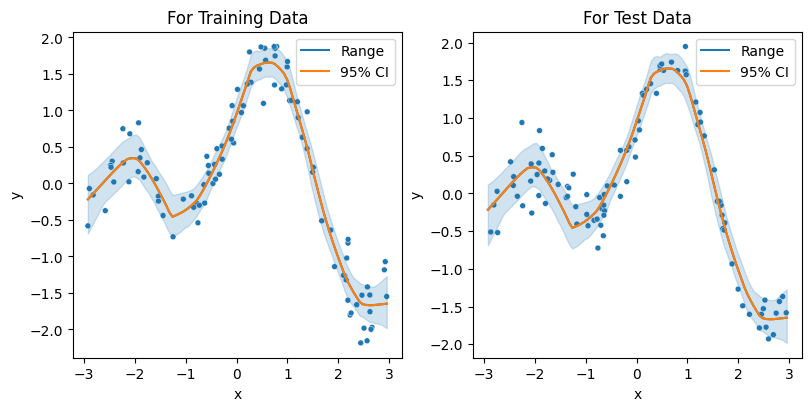
\includegraphics[width=0.45\textwidth]{images/hmc_bnn--problem_A--sb.png} & 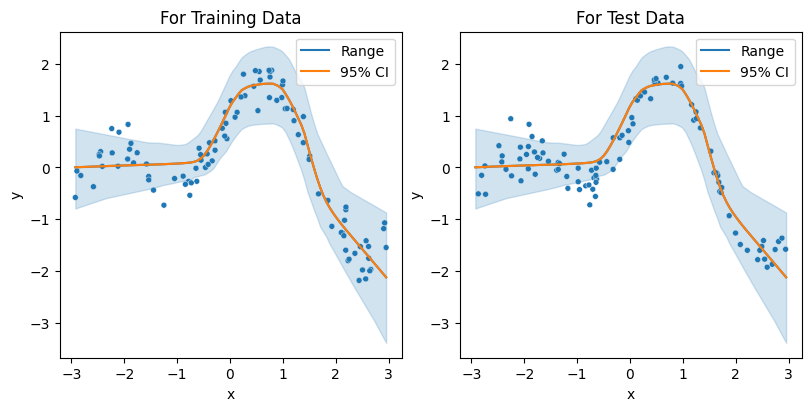
\includegraphics[width=0.45\textwidth]{images/vi_bnn--problem_A--sb.png}\\
(C) & 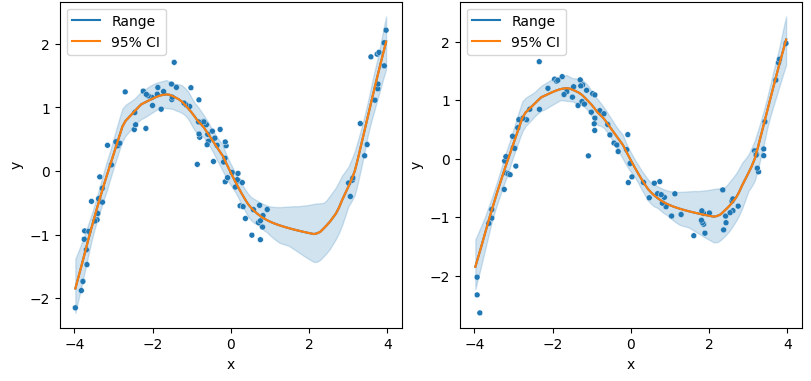
\includegraphics[width=0.45\textwidth]{images/hmc_bnn--problem_B--sb.png} & 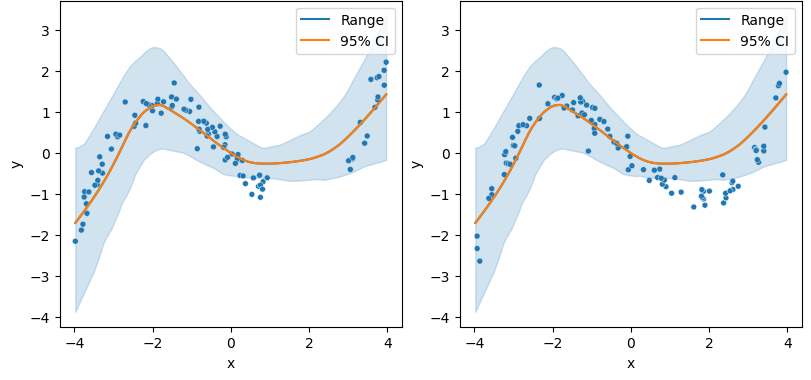
\includegraphics[width=0.45\textwidth]{images/vi_bnn--problem_B--sb.png}\\
(D) & 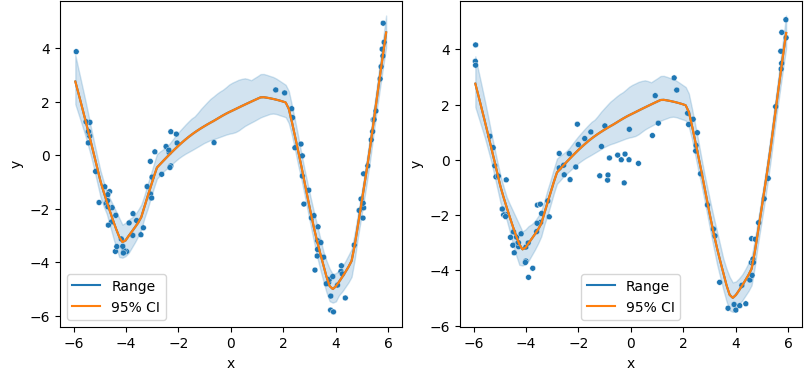
\includegraphics[width=0.45\textwidth]{images/hmc_bnn--problem_C--sb.png} & 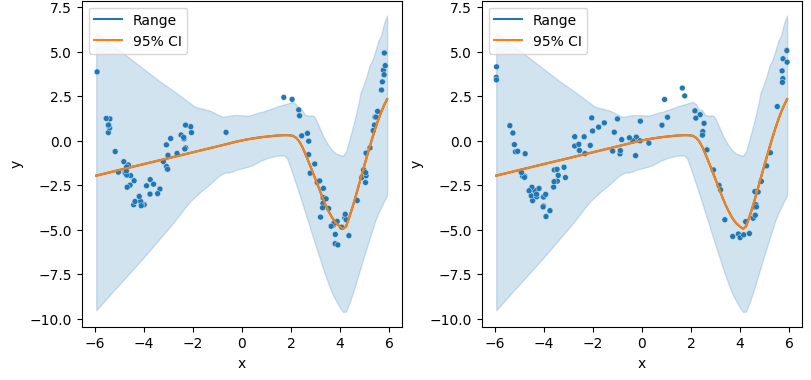
\includegraphics[width=0.45\textwidth]{images/vi_bnn--problem_C--sb.png}\\
 & 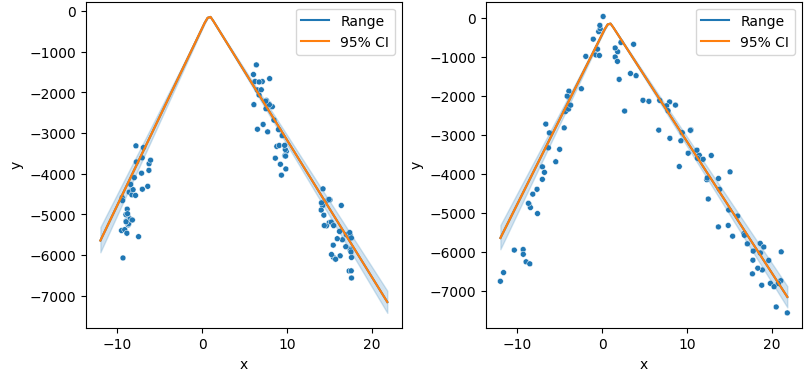
\includegraphics[width=0.45\textwidth]{images/hmc_bnn--problem_D--sb.png} & 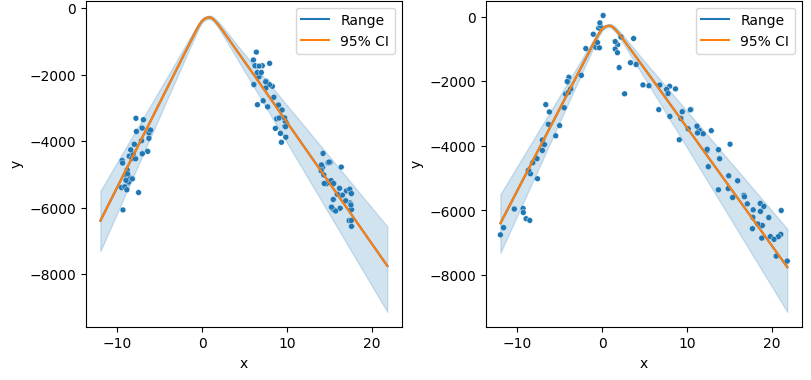
\includegraphics[width=0.45\textwidth]{images/vi_bnn--problem_D--sb.png}
\end{tabular}
\caption{HMC BNN \& VI BNN Performance (500 Epochs)}
\label{tbl:table_of_figures}
\end{table*}

\begin{table*}
\centering
\begin{tabular}{cccc}
(A) & (B) & (C) & (D)\\
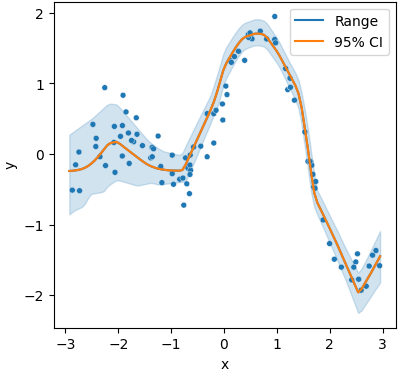
\includegraphics[width=0.21\textwidth]{images/vi_bnn--problem_A--sb--1500_epochs.png} & 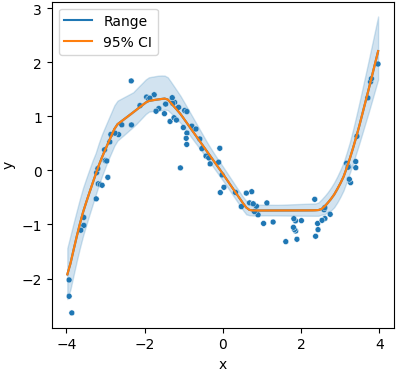
\includegraphics[width=0.21\textwidth]{images/vi_bnn--problem_B--sb--1500_epochs.png} & 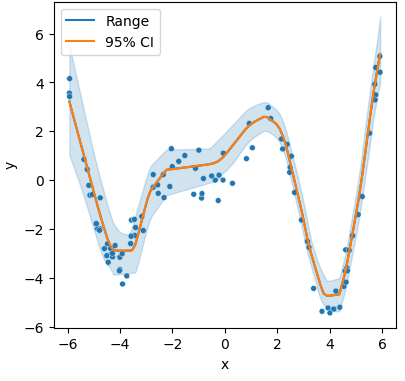
\includegraphics[width=0.21\textwidth]{images/vi_bnn--problem_C--sb--1500_epochs.png} & 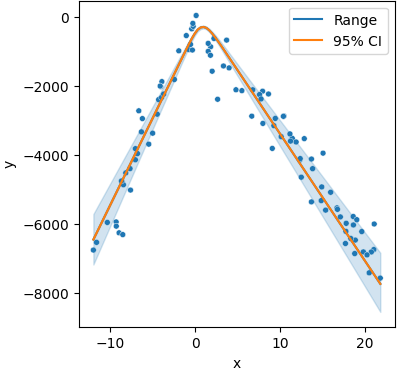
\includegraphics[width=0.21\textwidth]{images/vi_bnn--problem_D--sb--1500_epochs.png}
\end{tabular}
\caption{VI BNN Performance (1500 Epochs, Test Data Only)}
\label{tb2:table_of_figures}
\end{table*}


\begin{table*}
\centering
\begin{tabular}{cccc}
\textbf{HMC BNN} (A) & \textbf{VI BNN} (A) & \textbf{HMC BNN} (B) & \textbf{VI BNN} (B)\\
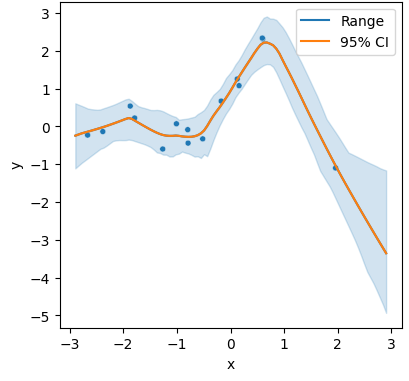
\includegraphics[width=0.21\textwidth]{images/hmc_bnn--problem_A--sb--sparse_data.png} & 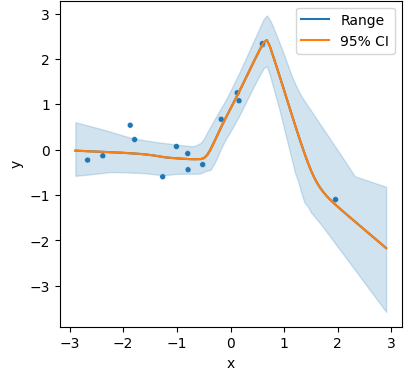
\includegraphics[width=0.21\textwidth]{images/vi_bnn--problem_A--sb--sparse_data.png} & 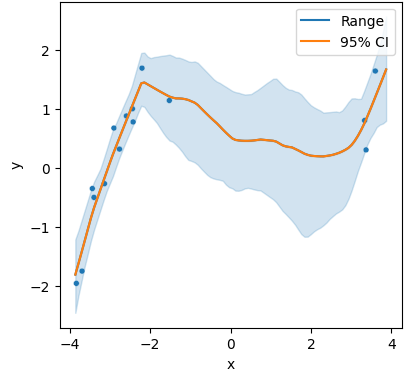
\includegraphics[width=0.21\textwidth]{images/hmc_bnn--problem_B--sb--sparse_data.png} & 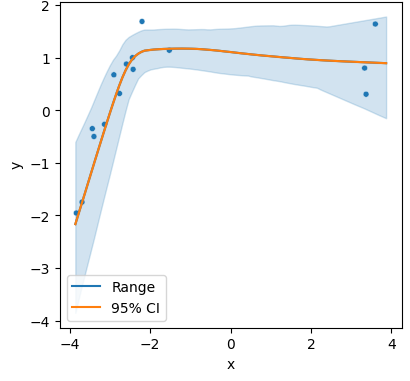
\includegraphics[width=0.21\textwidth]{images/vi_bnn--problem_B--sb--sparse_data.png}\\
\end{tabular}
\caption{HMC BNN \& VI BNN Performance (500 \& 1500 Epochs, Sparse Data)}
\label{tb3:table_of_figures}
\end{table*}

In the given graphs, the dots represent the synthetic data points, the blue area represents the range of variation in the model's predictions, and the orange area represents the $95\%$ confidence interval of the distribution of predictions. In each graph, the orange area is so close to the curve of average predictions that they are indistinguishable, which means most of the predictions are very close to the average.\\

The first set of experiments has the following training parameters for both models: $500$ epochs with batch size $32$ and learning rate $0.01$. These values were chosen as they achieved sufficient predictive accuracy for an ANN (without Bayesian layers). The models were trained for $100$ data points per problem. The results are presented in \textbf{Table I}, where each row represents result for one problem, starting from problem A at the top. Focusing on HMC BNN, the predictions show greater variation and hence more uncertainty when there are gaps or sparsity in the data, as seen in the intervals $[1, 3]$ for problem B and $[-2, 2]$ for problem B. In problem A, the predictions vary most at inflection points of the average prediction, where there is the greatest complexity in the data's distribution.\\

Turning to VI BNN, the poor average predictive accuract reveals that the number of epochs and/or batch size were insufficient for the model to properly train for the data. Nonetheless, it can observed that, unlike HMC BNN, the predictions do not show greater variation and hence uncertainty in gaps or sparsity, but instead show greater variation at the edges of the interval for which the data is defined, suggesting uncertainty about how the data extends beyond the given interval. In order to more effectively capture VI BNN's quantification of uncertainty, the VI BNN has been trained for $1500$ epochs. The results are presented in \textbf{Table II} (shown only for the test data), where the average predictive accuracy is comparable to that of HMC BNN. Again, the predictions do not show greater variation and hence uncertainty in gaps or sparsity. Only in problem A is there greater variation in the noisier part of the data, in the interval $[-3, -1]$. Moreover, training for more epochs (e.g. $2000$ epochs) tends to reduce the variation in predictions overall (see appendix E).\\

Observe that for both models in problem D, despite the presence of a gap in the data in the interval $[10, 14]$, both models show very low predictive uncertainty. To explore the cause, two experiments were run: (1) all the VI BNN's layers were set as Bayesian linear layers, and (2) a hidden Bayesian layer was added to the VI BNN in (1). The results of these experiments are given in appendix E.\\

In the next set of experiments, the models were trained for sparser data, i.e. $15$ data points per problem instead of $100$, without purposefully added gaps in the data. To achieve a comparable level of predictive accuracy, the functional model for HMC BNN and the VI BNN were trained for $500$ and $2000$ epochs respectively (batch size and learning rate being the same as before). The experiment was focused on problems A and B. The goal here was to test whether the models show greater predictive uncertainty due to the data's sparsity. The results are presented in \textbf{Table III}. In problem A and for both models, greater variation in predictions is observed where data is sparser, i.e. in the interval $[2, 3]$. In problem B, HMC BNN shows a much greater variation in predictions in the interval $[-2, 3]$, where there are no data points, which corresponds to a much greater uncertainty about its predictions in the absence of data. However, the variation in the predictions of VI BNN in problem B does not show the same correspondence between variation in the predictions and uncertainty about the predictions.

\section{Conclusion}
Given the domain of synthetic regression problems with single-valued inputs, the performance of HMC BNN aligns reasonably well with expectations about the predictive uncertainty of the model, which suggests that taking HMC samples from a trained ANN is a promising approach to quantifying a model's predictive uncertainty. To elaborate, the distribution of HMC samples for the ANN's hidden weights have been observed to correspond to the data's noise (e.g. in the interval $[-3, -1]$ in problem A), sparsity (e.g. in the results presented in \textbf{Table III}, and in the intervals $[1, 3]$ in problem B and $[-2, 2]$ in problem C, as presented in \textbf{Table I}), thereby showing correspondence between the distribution of HMC samples for the ANN's hidden weights and the epistemic uncertainty implicit in the ANN and the observed data.\\

An issue in the above conclusion, however, is the lack of a rigorous metric for evaluating the quality of the quantification of uncertainty. Thus, further work in exploring and applying such metrics to the BNN implementations would be a valuable step in more accurately evaluating the performance of these implementations (an attempted approach using KS-test to compare the expected distribution of the synthetic outputs to the distribution of predictions is presented in appendix F).\\

However, since only one layer of the model was distributed, the HMC samples are likely not representative of the distribution of potential parameterisations of the ANN as a whole, since for any ANN, there likely exists a variety of parameterisations that lead to accurate predictions, and the final parameterisation of the ANN after training is sensitive to the initialisation of the ANN's weights. In other words, since a set of trained weights can be reasonably assumed to represent a sample at or close to one of the posterior's mode (as indicated in \textit{2) HMC Sampler} from subsection \textit{B. HMC Implementation} from section \textbf{IV. Methodology}), the distribution of the hidden layer's weights while keeping other layers constant would not sufficiently explore the multi-modal posterior of the ANN's weights as a whole. Hence, valuable further work to more rigorously study the effectiveness of HMC in deep learning would be to develop an HMC BNN implementation that can sample for the weights of the whole model, as done by Brian and Da Veiga (2022).\\

The VI BNN implementation used, which is based on adversarial BNN, shows less consistent and overall poorer performance. This may be a deficiency in the particular approximate BI method used, and hence, no broader conclusion about the effectiveness of approximate BI methods can be made. Hence, further work would be valuable in exploring the effectiveness of other approximate BI methods, such as Bayes-by-Backpropagation and Monte Carlo Dropout.\\

\begin{thebibliography}{00}

\bibitem{Andrieu and Thoms, 2008} Andrieu, C. and Thoms, J. (2008). A tutorial on adaptive MCMC. \textit{Springer}. 18, pp. 343–373. doi:10.1007/s11222-008-9110-y.

\bibitem{Betancourt, 2018} Betancourt, M. (2018). A Conceptual Introduction to Hamiltonian Monte Carlo. \textit{arXiv preprint arXiv:1701.02434}.

\bibitem{Brian and Da Veiga, 2022} Brian, S. and Da Veiga, S. (2022). Benchmarking Bayesian neural networks and evaluation metrics for regression tasks. \textit{arXiv preprint arXiv:2206.06779}.

\bibitem{Carroll, 2019} Carroll, C. (2019). \textit{Hamiltonian Monte Carlo from scratch}. [online] Available from: \url{https://colindcarroll.com/2019/04/11/hamiltonian-monte-carlo-from-scratch} [Accessed 21 August 2024].

\bibitem{Chandra and Simmons, 2023} Chandra, R. and Simmons, J. (2023). Bayesian neural networks via MCMC: a Python-based tutorial. \textit{arXiv preprint arXiv:2304.02595}.

\bibitem{Cook, 2020} Cook, J. D. (2020). \textit{Leapfrog integrator}. [online] Available from: \url{https://www.johndcook.com/blog/2020/07/13/leapfrog-integrator/}.

\bibitem{Foong et al., 2019} Foong, A. Y. K., Burt, D. R., Li, Y. and Turner, R. E. (2019). On the Expressiveness of Approximate Inference in Bayesian Neural Networks. \textit{arXiv preprint arXiv:1909.00719}.

\bibitem{Ganguly and Earp, 2021} Ganguly, A. and Earp, S. W. F. (2021). An Introduction to Variational Inference. \textit{arXiv preprint arXiv:2108.13083}.

\bibitem{GeeksForGeeks, 2024} GeeksForGeeks. (2024). \textit{Kolmogorov-Smirnov Test (KS Test)}. [online] Available from: \url{https://www.geeksforgeeks.org/kolmogorov-smirnov-test-ks-test/} [Accessed 23 August 2024].

\bibitem{janosh.dev, 2019} janosh.dev (2019). \textit{Training BNNs with HMC}. [online] Available from: \url{https://janosh.dev/posts/hmc-bnn} [Accessed 21 August 2024].

\bibitem{Jospin et al., 2020} Jospin, L. V., Laga, H., Boussaid, F., Buntine, W. and Bennamoun, M. (2020). Hands-on Bayesian Neural Networks – A Tutorial for Deep Learning Users. \textit{arXiv preprint arXiv:2007.06823}.

\bibitem{Kim, 2020} Kim, H. (2020). \textit{Bayesian-Neural-Network-Pytorch}. [online] Available from: \url{https://github.com/Harry24k/bayesian-neural-network-pytorch} [Accessed 21 August 2024].

\bibitem{Lee et al., 2021} Lee, S., Kim, H. and Lee, J. (2021). GradDiv: Adversarial Robustness of Randomized Neural Networks via Gradient Diversity Regularization. \textit{arXiv preprint arXiv:2107.02425}.

\bibitem{Martin et al., 2021} Martin. O. A., Kumar, R. and Lao, J. Bayesian Modeling and Computation in Python. Boca Ratón, Florida, USA: CRC Press, Taylor \& Francis Group. ISBN: 978-0-367-89436-8.

\bibitem{Murphy, 2012} Murphy, K. P. (2012). '3. Generative models for discrete data'. \textit{Machine Learning: A Probabilistic Perspective}. London, England: The MIT Press. pp. 65-87.

\bibitem{Neal, 2011} Neal, R. (2011). 'Chapter 5: MCMC using Hamiltonian dynamics'. In: Brooks, S., Gelman, A., Jones, G., and Meng, X. \textit{Handbook of Markov Chain Monte Carlo}. Boca Ratón, Florida, USA: CRC Press, Taylor \& Francis Group. pp. 113-162.

\bibitem{Nowling, 2016} Nowling, R. J. (2016). \textit{Deriving the Leapfrog Integrator}. [online] Available from: \url{https://rnowling.github.io/math/2016/11/11/deriving-leapfrog.html} [Accessed 23 August 2024].

\bibitem{TensorFlow, 2023} TensorFlow. (2023). \textit{tfp.mcmc.SimpleStepSizeAdaptation}. [online] Available from: \url{https://www.tensorflow.org/probability/api_docs/python/tfp/mcmc/SimpleStepSizeAdaptation} [Accessed 21 August 2024].

\bibitem{Wikipedia, 2024} Wikipedia. (2024). \textit{Leapfrog integration}. [online] Available from: \url{https://en.wikipedia.org/wiki/Leapfrog_integration} [Accessed 23 August 2024].

\bibitem{Yao et al., 2019} Yao, J., Pan, W., Ghosh, S. and Doshi-Velez, F. (2019). Quality of Uncertainty Quantification for Bayesian Neural Network Inference. \textit{arXiv preprint arXiv:1906.09686}.

\bibitem{Zaiontz, 2024} Zaiontz, C. \textit{One-Sample Kolmogorov-Smirnov Table}. [online] Available from: \url{https://real-statistics.com/statistics-tables/kolmogorov-smirnov-table/} [Accessed 23 August, 2024].

\end{thebibliography}
\vspace{12pt}

\textit{(The appendix starts from the next page)}

\clearpage

\section*{Appendix}

\par\noindent\rule{0.49\textwidth}{0.1pt}

\subsection*{Appendix A: Use of Negative Log-Probability in HMC}
Let $\theta = (\theta_1, \theta_2 ... \theta_k)$ be a parameterisation of a given generative model. Let $m$ be the momentum, where $m = (m_1, m_2 ... m_k)$ (each $m_i$ being the momentum in the $i$th dimension). Also, note that $P(\theta, m) = P(\theta|D)P(m)$, which means $\log P(\theta, m) = \log (P(\theta|D) P(m)) = \log P(\theta|D) + \log P(m)$. Hence:

\begin{equation*}
	- \log P(\theta, m) = - \log P(\theta|D) - \log P(m)
\end{equation*}

This is of the form $H(\theta, m) = K(\theta) + V(\theta)$, where $H(\theta, m) = - \log P(\theta, m)$ (Hamiltonian),  $K(m) = - \log P(m)$ ("kinetic energy"), and $V(\theta) = - \log P(\theta|D)$ ("potential energy"). Thus, we have Hamilton's equations:

\begin{equation*}
	\frac{d \theta}{dt} = \frac{\delta H}{\delta m}, \text{ } \frac{dm}{dt} = - \frac{\delta H}{\delta \theta}
\end{equation*}

Hamilton's equations describe the state of a physical system with one body of a fixed mass moving in a space of $k$ dimensions ($k \geq 1$). Now, even though Hamilton's equations were meant to deal with physical spaces, we can accurately extend their application to analogous simulated or abstract spaces, such as a high-dimensional parameter space of a Bayesian model.\\

In the context BI, the "position" of the sample can be thought of as the location of a particle, and the "momentum" provides the force needed to move the particle through the parameter space of the distributions. As shown above, the Hamiltonian for BI has the negative log-probability of the posterior. However, since the negative log-probability preserves the distribution of the posterior's probability mass as well as the posterior's modes (albeit that the modes are represented by minima instead of maxima), samples from the the negative log-probability of the posterior follow the same distribution as samples the posterior. Hence, Hamilton's equations provide a valid means to explore the posterior.

\par\noindent\rule{0.49\textwidth}{0.1pt}

\subsection*{Appendix B: Reasoning for HMC's Acceptance Criterion}
The HMC algorithm is given below is drawn mostly from Carroll (2019) with changes made to more closely reflect the mathematics behind the algorithm. The names and symbols used are explained in the table after the algorithm:\\

\begin{algorithm}{H}
\textbf{input} $n, -\log p, \theta_0, T, \Delta t$
\caption{Run HMC Sampler}
\begin{algorithmic}[H]
\State $\text{samples} \gets \text{array of size } n$
\State $g \gets \text{grad}(-\log p)$
\For{$i \in (0, 1, 2 ... n-1)$}                
    \State $m_0 \gets \text{draw}(\mathcal{N}(0, \sigma I))$
    \State $\theta_T, m_T \gets \text{leapfrog}(\theta_0, m, g, T, \Delta t)$
    \State $H_\text{old} \gets -\log(p)(\theta_0) - \log \mathcal{N}(0, \sigma I)(m_0)$
    \State $H_\text{new} \gets -\log(p)(\theta_T) - \log \mathcal{N}(0, \sigma I)(m_T)$
    \State $\alpha \gets e^{H_\text{old} - H_\text{new}}$
    
    \If{$\text{draw}(\mathcal{U}(0, 1)) < \alpha$}
        \State $\text{samples}[i] \gets \theta_T$
    \Else
        \State $\text{samples}[i] \gets \theta_0$
    \EndIf
\EndFor
\end{algorithmic}
\textbf{return} $\text{samples}$
\end{algorithm}

\begin{tabular}{| m{1.5cm} | m{6cm} |}
    \hline
    $n$ & Number of samples to draw\\
    \hline
    $p$ & Target probability distribution\\
    \hline
    $-\log p$ & Negative log-probability of $p$\\
    \hline
    $T, \Delta t$ & Number and size of leapfrog steps\\
    \hline
    $\theta_0, m_0$ & Current position and momentum\\
    \hline
    $\theta_T, m_T$ & Proposed position and momentum\\
    \hline
    $\alpha$ & Acceptance probability of proposal\\
    \hline
    $H_\text{old}$ & Hamiltonian function for $\theta_0, m_0$\\
    \hline
    $H_\text{new}$ & Hamiltonian function for $\theta_T, m_T$\\
    \hline
    $\mathcal{N}(\mu, \sigma)$ & Normal distribution\\
    \hline
    $\mathcal{U}([a, b])$ & Uniform distribution\\
    \hline
    $\text{grad}$ & Returns callable gradient\\
    \hline
    $\text{draw}$ & Function to draw from given distribution\\
    \hline
    $\text{leapfrog}$ & Leapfrog integrator\\
    \hline
\end{tabular}\\~\\

HMC can be explained using a physical analogy, wherein $-\log p$ defines the contours of a force field (e.g. a gravitational field) along which a body — the sampler, in our case — can travel, with each position representing a sample. Starting from the current position $\theta_0$, the leapfrog integrator is a symplectic integrator that uses the gradient of $-\log p$ and the current momentum $m_0$ to simulate the exact trajectory of the sampler along the contours of $-\log p$ for $L = \frac{T}{\Delta t}$ discrete time steps. Thus, a symplectic integrator discretises the Hamiltonian equations used to explore the posterior. If the momentum is well-chosen, the trajectory travels through positions with the same or similar acceptance probabilities as the current position.\\

However, despite its accuracy, a symplectic integrator is likely to introduce at least some errors in the calculation of trajectories (Betancourt, 2018). Furthermore, the momentum may be sub-optimal. To account for such errors, a proposed sample is accepted based on the Metropolis criterion, i.e. a proposed sample is accepted with the acceptance probability $\alpha = \min(1, e^{H_\text{old} - H_\text{new}})$ (Neal, 2011). The mathematical details and reasoning are given in the following paragraphs.\\

Let $\theta$ be the current position (i.e. the current state of the Markov chain sampling the Bayesian model's parameterisations). Let $m$ be the current momentum. Likewise, let $\theta^*$ and $m^*$ be the proposed position and momentum. Also, let $H(\theta, m)$ be the Hamiltonian for position $\theta$ and momentum $m$. Then, we have the following cases:\\

\begin{itemize}
	\item $e^{H(\theta, m) - H(\theta^*, m^*)} \geq 1 \implies H(\theta^*, m^*) \geq H(\theta, m)$
	\item $e^{H(\theta, m) - H(\theta^*, m^*)} \leq 1 \implies H(\theta^*, m^*) \leq H(\theta, m)$\\
\end{itemize}

$H(\theta^*, m^*) \geq H(\theta, m)$ means the proposed state is from a region in the posterior of equal or higher probability mass, which means it should always be accepted, because we want to sample more from regions of equal or higher probability mass. $H(\theta^*, m^*) < H(\theta, m)$ means the proposed state is from a region of lower probability mass, which means it should be accepted only probabilistically, with the probability of accepting it being proportional to its closeness to the current state (in terms of probability density), because we want there to be a lower but non-zero chance of sampling from a sparser region after sampling from a denser region, with the condition that the lower the density, the lower the chance.

\par\noindent\rule{0.49\textwidth}{0.1pt}

\subsection*{Appendix C: Leapfrog Integration}
Leapfrog integration is a method for numerically any integrating differential equations (DE) of the form $\frac{d^2x}{dt^2} = f(x)$, i.e. $x'' = f(x)$ (Wikipedia, 2024). Here, $x$ is a function of $t$ (typically, $x$ is position and $t$ is time). In general, integrating a DE means solving it, i.e. finding the functions for the differentials so as to satisfy the DE. In the case of leapfrog integration, integrating a DE of the form $x'' = f(x)$ means solving for the function $x$ (note that $f$ is given). More precisely, for discrete steps along $t$, the leapfrog integrator tries to approximate the values for $x$ across for a given number of steps. Typically, $x$ is position and $t$ is time; this analogy can be extended to any use-case.\\

To clarify, note the following: (1) $x$ is a function of $t$, (2) we are dealing with a $k$-dimensional space, where $k \geq 1$, and hence, (3) if $x(t)$ is the position, it would be an array of coordinates. Leapfrog integration is used when there is no analytical equation for $x(t)$ that satisfies the DE, or at least when the analytical equation is too complex to derive; the idea is to use a numerical integration algorithm to compute values of $x(t)$ on discrete time steps $\Delta t$. In the following equations, we can see how the values are approximated for $x$. The complete derivation is based on the derivation presented by Nowling (2016), with the notation modified according to the algorithm presented by Cook (2020). Note that here, we are using the analogy (which can be accurately translated to posterior sampling) of $x$ as position, $v$ as velocity, $a$ as acceleration and $t$ as time. The algorithm is as follows:\\

\begin{enumerate}
	\item Calculate $a$ for the current time step
	\item Calculate $x$ for the next time step
	\item Calculate $a$ for the next time step
	\item Calculate $v$ for the next time step\\
\end{enumerate}

Mathematically, the above steps are:\\

\begin{enumerate}
	\item $a(t) = -f(x(t))$
	\item $x(t + \Delta t) = x(t) + v(t)\Delta t + \frac{1}{2}a(t)\Delta t^2$
	\item $a(t + \Delta t) = -f(x(t+\Delta t))$
	\item $v(t + \Delta t)=v(t) + \frac{1}{2}(a(t) + a(t + \Delta t))\Delta t$\\
\end{enumerate}

Here, $x$, $v$ and $a$ are related as follows:\\

\begin{itemize}
	\item $x''(t) = a(t) = f(x)$
	\item $v''(t) = a'(t)$
	\item $x''(t) = v'(t) = a(t)$
	\item $x'(t) = v(t)$\\
\end{itemize}

The above relationships can be easily understood if one considers $x$ as position, $v$ as velocity, $a$ as acceleration, and $t$ as time. Note that position, velocity and acceleration are all represented by vectors if the number of spatial dimensions are greater than one.

\par\noindent\rule{0.49\textwidth}{0.1pt}

\subsection*{Appendix D: VI with Evidence Lower Bound (ELBO)}
KL-divergence is a well-established measure of distance used in VI. If used, the optimisation function would based on the KL-divergence between $q_\phi(\theta)$ and $p = P(\theta|D)$. Given that $\Theta$ is the set of all hypothetical parameterisations of a given model, the KL-divergence between $q_\phi(\theta)$ and $P(\theta|D)$ is given by the following:

\begin{equation*}
	KL(q_\phi(\theta) || P(\theta|D))
	= \int_{\theta \in \Theta} q_\phi(\theta) \log \frac{q_\phi(\theta)}{P(\theta|D)} d\theta
\end{equation*}\\

However, $P(\theta|D)$ is the posterior being approximated and thus cannot be in the optimisation function. But there exists a function derived from KL-divergence, namely the Evidence Lower Bound (ELBO), that uses only the variational distribution $q_\phi$ and the joint distribution $P(\theta, D) = P(D|\theta)|P(\theta)$, i.e. the unnormalised posterior. Note that these distributions are known, since $q_\phi$ and the prior $P(\theta)$ are chosen and since the likelihood $P(D|\theta)$ is based on a chosen generative model. Mathematically, ELBO is given as follows (Jospin et al., 2020):

\begin{equation*}
	\int_{\theta \in \Theta} q_\phi(\theta) \log \frac{p(\theta, D)}{q_\phi(\theta)} d\theta
\end{equation*}\\

ELBO is derived such that maximising it achieves the same optimisation as minimising KL-divergence. In practice, the above integral is estimated through numerical methods, e.g. averaging Monte Carlo samples drawn from the variational and joint distributions and plugging them into the ELBO formula\footnote{Here, the integral becomes a summation.} (Martin et al., 2021). For the derivation of ELBO, check \href{https://github.com/pranigopu/mastersProject/tree/main/conceptual-notes/bayesian-inference/sampling-methods/variational-inference-vi}{\textit{conceptual-notes/bayesian-inference/sampling-methods/variational-inference-vi}} in \href{https://github.com/pranigopu/mastersProject}{\textit{github.com/pranigopu/mastersProject}}, the repository associated with this paper.

\par\noindent\rule{0.49\textwidth}{0.1pt}

\subsection*{Appendix E: Results of Further Experiments}
\subsubsection{VI BNN Trained for 2000 Epochs}
The following set of graphs are to demonstrate that increasing the number of training epochs for the VI BNN implementation used tends to decrease the variation in its predictions, which means it likely does not quantify predictive uncertainty more effectively with more training epochs.

\begin{table}[H]
\centering
\begin{tabular}{cc}
(A) & (B)\\
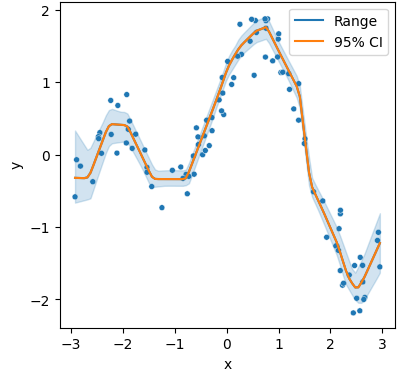
\includegraphics[width=0.21\textwidth]{images/vi_bnn--problem_A--sb--2000_epochs.png} & 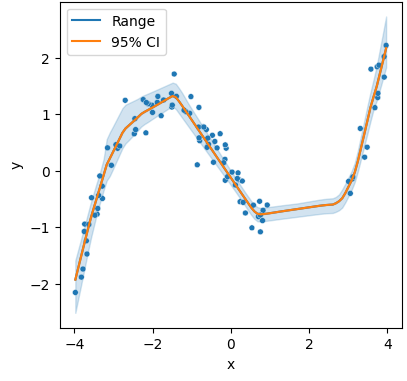
\includegraphics[width=0.21\textwidth]{images/vi_bnn--problem_B--sb--2000_epochs.png}\\
(C) & (D)\\
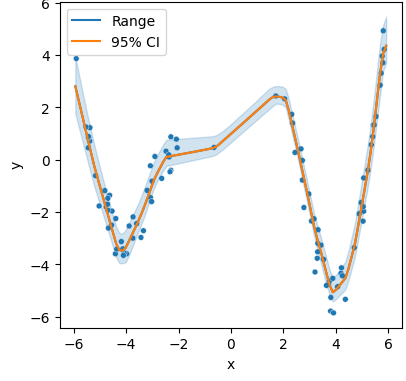
\includegraphics[width=0.21\textwidth]{images/vi_bnn--problem_C--sb--2000_epochs.png} & 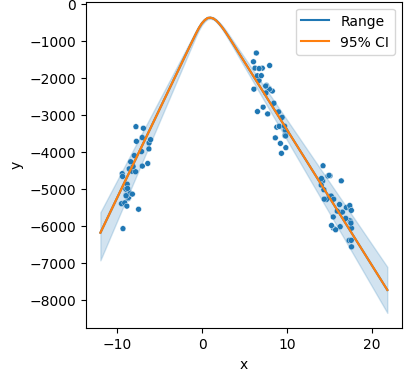
\includegraphics[width=0.21\textwidth]{images/vi_bnn--problem_D--sb--2000_epochs.png}
\end{tabular}
\caption{VI BNN Performance (2000 Epochs, Training Data Only)}
\label{tb4:table_of_figures}
\end{table}

\subsubsection{VI BNN Experiments for Problem D}
The following graphs are the result of running VI BNN with all its layers set as Bayesian linear layers. Two architectures were tried, with one and two hidden layers respectively.

\begin{table}[H]
\centering
\begin{tabular}{cc}
\textbf{1 Hidden Layer} & \textbf{2 Hidden Layers}\\
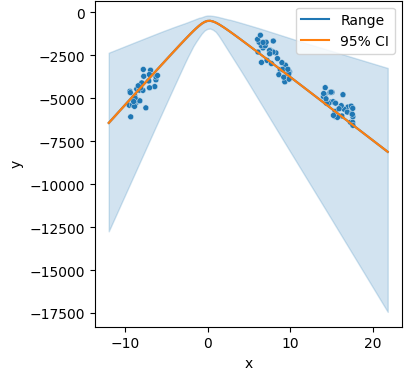
\includegraphics[width=0.21\textwidth]{images/vi_bnn--problem_D--sb--full_bayesian.png} & 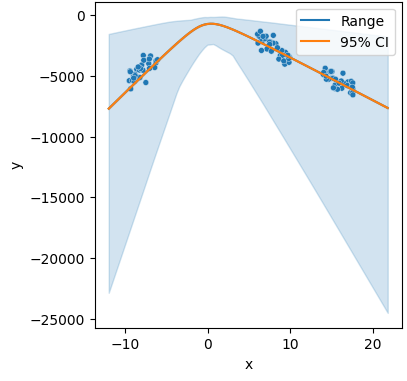
\includegraphics[width=0.21\textwidth]{images/vi_bnn--problem_D--sb--full_bayesian--2_hidden_layers.png}
\end{tabular}
\caption{VI BNN for Problem D (Full Bayesian, Training Data Only)}
\label{tb5:table_of_figures}
\end{table}

As can be observed, the quantification of the predictive uncertainty for the gap in the data does not improve. This could be an issue with the particular form of VI BNN used, in which case uncertainty quantification may improve if more complex architectures were used for HMC BNN.

\par\noindent\rule{0.49\textwidth}{0.1pt}

\subsection*{Appendix F: KS-Test for Expected and Predicted Outputs}
Based on the way the synthetic regression problems are defined, every input data point, i.e. every $x_i$, is associated with a range of possible outputs; these outputs are distributed based on the distribution of the error term. To be more precise, take a synthetic regression problem $y_i = g(x_i) + \epsilon_i$, where $g$ is some function of $x_i$ and $\epsilon \sim \mathcal{N}(0, \tau)$ is the error term (where $\mathcal{N}(\mu, \sigma)$ denotes a normal distribution with mean $\mu$ and standard deviation $\sigma$). Given an input $x_i$, the mean of the distribution of possible $y_i$ values is given by $g(x_i)$, which means $y_i \sim \mathcal{N}(g(x_i), \tau)$.\\

By the nature of BNNs, for each input data point, the BNN produces a range of predictions. Hence, it is reasonable to assume that if the likelihood and prior of the BNN are appropriately defined, and if the BI inference method is effective, then the distribution of predictions for each given input data point should match the theoretical distribution of outputs $\mathcal{N}(g(x_i), \tau)$. This is the basis for the Kolmogorov-Smirnov (KS) test, specifically the KS-test between the theoretical distribution of outputs and the empirical distribution of predictions. This may be a way to test the validity of a BNN implementation.\\

The KS-test used here would be a one-sample KS-test, the sample being the empirical distribution of predictions. The KS-test is based on the Kolmogorov distribution, which represents the cumulative distribution function (CDF) of the maximum difference between the sample empirical distribution and the CDF of the reference (theoretical) distribution (GeeksForGeeks, 2024). The probability distribution function (PDF) of the Kolmogorov distribution itself is not expressed in an analytical form. Instead, tables or statistical software are used to obtain critical values. The distribution is influenced by sample size, and the critical values depend on the significance level chosen for the test (GeeksForGeeks, 2024).\\

\begin{table}
\begin{tabular}{cc}
\textbf{HMC BNN} & \textbf{VI BNN}\\
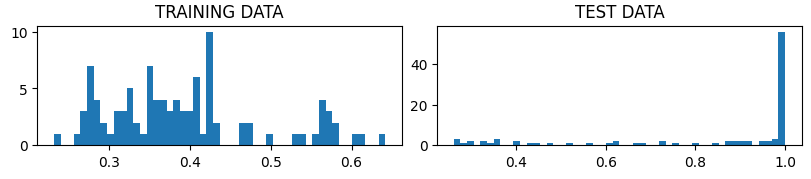
\includegraphics[width=0.21\textwidth]{images/ks_test--hmc_bnn--problem_A.png} & 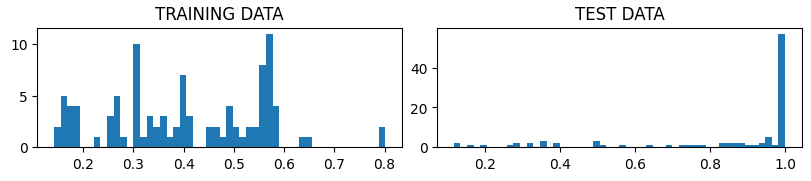
\includegraphics[width=0.21\textwidth]{images/ks_test--vi_bnn--problem_A.png}\\ 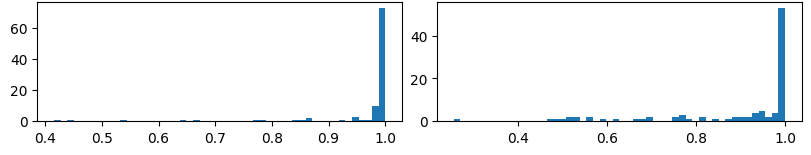
\includegraphics[width=0.21\textwidth]{images/ks_test--hmc_bnn--problem_B.png} & 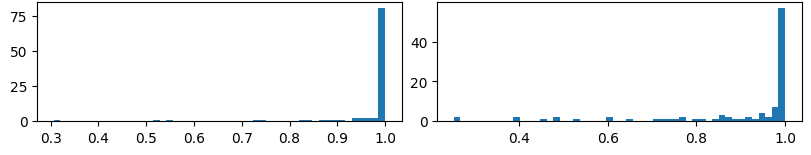
\includegraphics[width=0.21\textwidth]{images/ks_test--vi_bnn--problem_B.png}\\
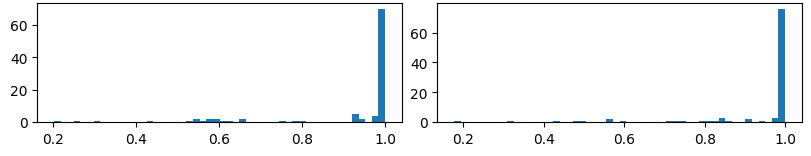
\includegraphics[width=0.21\textwidth]{images/ks_test--hmc_bnn--problem_C.png} & 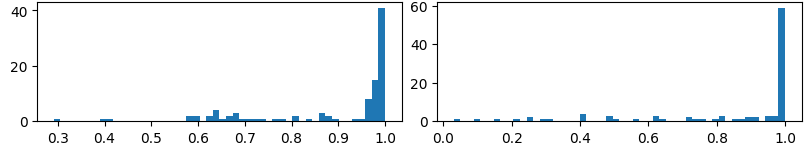
\includegraphics[width=0.21\textwidth]{images/ks_test--vi_bnn--problem_C.png}\\
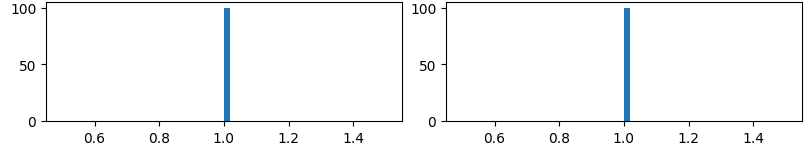
\includegraphics[width=0.21\textwidth]{images/ks_test--hmc_bnn--problem_D.png} & 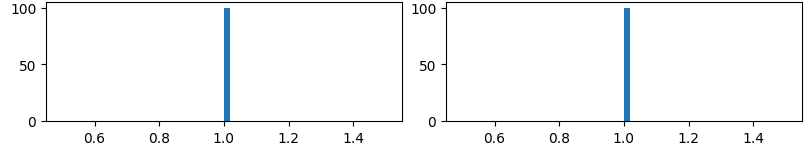
\includegraphics[width=0.2\textwidth]{images/ks_test--vi_bnn--problem_D.png}\\
\end{tabular}
\caption{KS-Statistic Histograms}
\label{tb5:table_of_figures}
\end{table}

Presented in \textbf{Table VI} are the histograms of the KS-statistic values obtained for all the input values (training and test inputs) of each problem (problems A-D from ordered from top to bottom). The number of samples is taken as $11000$; the acceptance rates of each run of HMC sampling for each problem was around $55\%$, and the total number of samples was $20000$, hence around $11000$ samples exist for each set of HMC BNN predictions, and accordingly, around $11000$ predictions were generated for each problem from the trained VI BNN model. Hence, given a significance level of $0.05$, the critical value of the KS-statistic is around $0.012$, based on calculations using the table given by Zaiontz (2024).\\

Importantly, the KS-test is a hypothesis test, with its null hypothesis being that there is no difference between the sample distribution and the reference distribution. If the KS-statistic exceeds the critical value, the null hypothesis is rejected. Hence, upon comparing the critical value $0.012$ to the presented results, it follows that practically none of the distributions of predicted outputs may be said to match the expected distributions of outputs.\\

\end{document}

